{

\setlength{\parindent}{0pt}
\setlength{\parskip}{1em}

\section{Preliminaries}
\glsfirst{ai}
\gls{ai}
\gls{ml}
\gls{bubu}
\gls{biba}
\subsection{Background}
\subsubsection{Satellite imagery for weather observation}
OOV CUBE has only 3 channel camera, but the efficient cloud segmentation requires 4th NIR channel. \todo{expplain why}
\subsubsection{State-of-the-art CNNs for Cloud Image Segmentation}

CNNs are a class of neural networks that apply small, learnable filters --- known as convolutional kernels --- across an image to extract spatial features. A CNN typically consists of multiple convolutional layers stacked sequentionally. Each layer applies a set of filters that capture different visual patterns, such as edges or textures. As the network goes deeper, the spatial resolution of the image decreases, while the depth (i.e., number of channels) increases. This is a result of applying multiple filters and optionally using pooling layers, which downsample feature maps to reduce computational complexity and introduce spatial invariance.
\todo{Explain briefly how they learn and optimize themselves, and what distinguishes them from just applying filters}
In image segmentation tasks such as cloud detection, preserving spatial resolution is critical. Therefore, architectures often include an upsampling mechanism to reconstruct high-resolution output from compressed feature representations. This is achieved through transposed convolution (also known as deconvolution). While standard convolution reduces spatial resolution by aggregating local pixel values, transposed convolution performs the reverse: it distributes each value in the smaller feature map across a larger output, effectively increasing spatial dimensions and reversing the compression.

One of the most influential architectures for image segmenation is the U-Net. Originally introduced by Ronneberger et al.~\cite{ronneberger2015u} for biomedical image segmentation, U-Net has become a standard in many domains, including remote sensing and cloud detection. A U-Net consists of an encoder-decoder structure. The encoder compresses the input image spatially while increasing its feature dimensionality. The decoder then reconstructs the spatial dimensions, progressively reducing the number of channels. This results in output imgage, that has the same spatial dimensions height and width, but could have a various number of channels, depending on the perceived task. The U-Net architecture shown in the diagram 1 was used by Mohajerani et al.~\cite{mohajerani2019cloudnet}  for their cloud detection algorithm.

\begin{figure}[H]
  \centering
  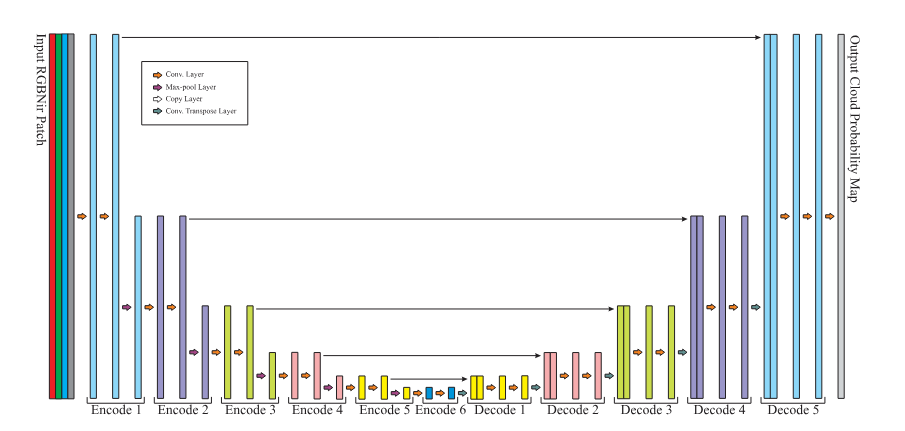
\includegraphics[width=\textwidth]{files/U-Net_cloud_detection.png}
  \caption{U-Net architecture adapted for cloud detection as used by Mohajerani et al.~\cite{mohajerani2019cloudnet}.}
  \label{fig:unet-architecture}
\end{figure}


A key innovation in U-Net is the use of residual (skip) connections \cite{he2015deepresiduallearningimage}, which dierectly link feature maps from the encoder to corresponding layers in the decoder with the same spatial size. These connections preserve fine-grained spatial details and significantly enhance segmentation quality. Moreover, they mitigate the vanishing gradient problem, facilitating the training of deeper networks and improving convergence.

\subsubsection{38-Cloud Landsat 8 dataset}

Landsat 8 is an Earth observation satellite launched on February 11, 2013, providing high-resolution multispectral imagery, including visible, near infrared (NIR), and thermal infrared bands \cite{landsat8}. For cloud segmentation tasks, the red, green, blue (RGB) and NIR channels are particularly valueable due to their ability to capture both visual and athmospheric information.

This thesis utilizes a dataset consisting of 38 annotated satellite images from the Landsat 8 mission, commonly referred to as the 38-Cloud dataset \cite{38cloud}. The dataset has been introduced and adapted in the following scientific publications \cite{CloudNet2019}, \cite{CloudDet2018}. Each image contains four spectral channels (RGB and NIR), along with a manually annotated dround truth mask that labels cloud pixels at the pixel level.

The dataset is divided into a training set containing 18 scenes and a test set with the remaining 20 scenes.

\subsubsection{Google Coral Dev Board Mini and Edge TPU}

Running machine learning inference on embedded systems is referred to as edge inference. The Coral dev Board Mini, developed by Google, is a compact single-board computer designed for such edge AI applications. It features quad-core MediaTek 8167s System-on-a-Chip (SoC) on the Armv8-A architecture, along with a dedicated Edge TPU – a hardware accelerator optimized for executing TensorFlow Lite models using 8-bit integer operations.

The Edge TPU delivers up to 4 trillion operations per second (TOPS) of performance while consuming only around 2 watts of power, making it ideal for use in resource-constrained environments such as satellites, where energy efficiency and reliability are crucial.

To deploy a model on Edge TPU, it must meet the following requirements:
\begin{itemize}
    \item Tensor parameters quantized
    \item Tensor sizes are constant at compile-time
    \item Model parameters (such as bias tensors) are constant at compile-time
    \item Tensors are either 1-, 2-, or 3-dimensional. If a tensor has more than 3 dimensions, then only the 3 innermost dimensions may have a size greater than 1.
    \item The model uses only the operations supported by the Edge TPU (see table 1 below). \todo{CROP the table to only relevant commands and paste it}
\end{itemize}

These requirements directly affect model architecture, training strategy, and tooling. For instance, certain operations unsopported by Edge TPU must be avoided, and quantization aware training or post-training quantization must be considered early in the development process.

The following image from Coral documentation summarizes the model conversion and deployment workflow.

\begin{figure}[H]
  \centering
  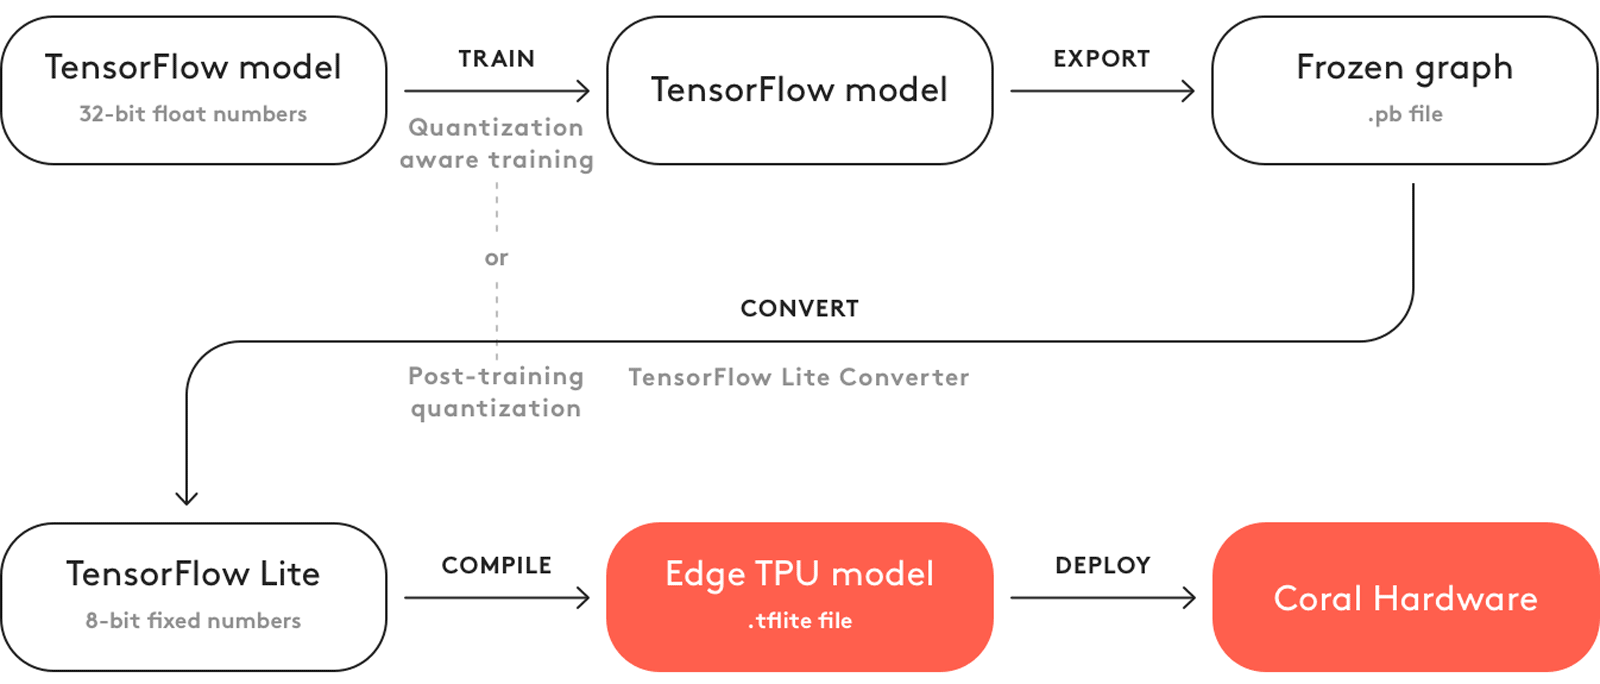
\includegraphics[width=\textwidth]{files/Edge_TPU_quantization.png}
  \caption{The basic workflow to create a model for the Edge TPU}
  \label{fig:quantization-chart}
\end{figure}

\subsubsection{Quantization}

Quantization is a mathematical method that maps a large set of (typically continuous) values to a smaller, discrete and countable set. Its first practical application can be traced back to 1957, in the context of pulse-code modulation within the field of signal processing. The earliest formal scientific documentation of the method appears in a publication from 1982, which is based on a draft manuscript originally authored in 1957. \cite{firstQuantization}

This technique is now widely employed in machine learning, where it is applied to the model weights and activations \cite{MLQuantization1}, \cite{MLQuantization2}. Quantization significantly reduces model size by compressing numerical precision, typically at the cost of a controlled reduction in accuracy. Two primary quantization methods are commonly used: general asymmetric zero-point quantization, and its special case --- symmetric absolute maximum (absmax) quantization. In the context of this work, the general asymetric approach is of primary importance.

To perform quantization, the boundaries \( x_{\text{min}} \) and \( x_{\text{max}} \) of the original (floating-point) range, and \( q_{\text{min}} \) and \( q_{\text{max}} \) of the target (quantized) value set must be defined. Once these are known, the corresponding scale and zero-point parameters are computed according to the following equations:

\begin{equation}
\text{scale} = \frac{x_{\text{max}} - x_{\text{min}}}{q_{\text{max}} - q_{\text{min}}}
\label{eq:scale}
\end{equation}

\begin{equation}
\text{zero-point} = \text{round}\left( q_{\text{min}} - \frac{x_{\text{min}}}{\text{scale}} \right)
\label{eq:zeropoint}
\end{equation}

With these parameters determined, input value \( x \) can be transformed into quantized form \( q_{\text{x}} \) and subsequently dequantized to an approximate value \( x_{\text{q}} \) using the following formulas:

\begin{equation}
q_{\text{x}} = \text{round}\left(\frac{x}{\text{scale}} \right) + \text{zero-point}
\label{eq:quantize}
\end{equation}

\begin{equation}
x_{\text{q}} \approx \left( q_{\text{x}} - \text{zero-point} \right) \cdot \text{scale}
\label{eq:dequantize}
\end{equation}

It is essential to note that both the scale and zero-point must be preserved in order to carry out the quantization and dequantization processes. For every value range subject to quantization, a unique pair of these parameters exists.

The following example demonstrates the use of zero-point quantization. Consider a set of continuous values ranging from -9.75 to 3.00. To map this range onto a discrete set defined by the integer interval [-128, 127], the scale and zero-point are calculated using equations \ref{eq:scale} and \ref{eq:zeropoint}:

\begin{equation*}
\text{scale} = \frac{3.00 - (-9.75)}{127 - (-128)} = 0.05
\end{equation*}

\begin{equation*}
\text{zero-point} = \text{round}\left( -128 - \frac{-9.75}{\text{scale}} \right) = 67
\end{equation*}


After this step, every value from the original dataset can be represented by its corresponding quantized counterpart. The following equations illustrate the quantization and subsequent dequantization of four examples using \ref{eq:quantize} and \ref{eq:dequantize}: \( x = 0 \), \( x = 3.00 \), \( x = 2.98 \), \( x = 2.95 \):

\begin{align*}
q_{0} &= \text{round}\left(\frac{0}{0.05} \right) + 67 = 67
& \quad
x_{67} &\approx \left( 67 - 67 \right) \cdot 0.05 = 0
\end{align*}

\begin{align*}
q_{3.00} &= \text{round}\left(\frac{3.00}{0.05} \right) + 67 = 127
& \quad
x_{127} &\approx \left( 127 - 67 \right) \cdot 0.05 = 3.00
\end{align*}

\begin{align*}
q_{2.98} &= \text{round}\left(\frac{2.98}{0.05} \right) + 67 = 127
& \quad
x_{127} &\approx \left( 127 - 67 \right) \cdot 0.05 = 3.00
\end{align*}

\begin{align*}
q_{2.95} &= \text{round}\left(\frac{2.95}{0.05} \right) + 67 = 126
& \quad
x_{126} &\approx \left( 126 - 67 \right) \cdot 0.05 = 2.95
\end{align*}

The last three examples implicitly 	demonstrate the loss of precision introduced by quantization. In this particular case, any input value between 2.95 and 3.00 will be represented, after conversion, by one of these two discrete values.

It is important to emphasize that the scale parameter etirely defines the quantizer's precision, under the assumption that the bit-width (i.e., 255 discrete representable values) is fixed, as well as the floating-point range from -9.75 to 3.00 being evenly distributed across the entire interval and free of outliers.

In practice, more advanced quantization techniques may be employed, such as outlier-aware clipping, per-axis and per-tensor quantization, symmetric and asymmetric schemes, or methods like dynamic range adjustment and mixed-precision quantization. However, the detailed explanation of these techniques falls outside the scope of this thesis.


\subsection{Concept}

\subsubsection{Data Preparation}

To efficiently utilize TensorFlows dataset loading and preprocessing capabilities, a versatile data handling method is implemented. A core idea behind this approach is to unify the preparation of training, validation and test subsets within a single configurable function. This function must manage all aspects of dataset construction and transformation according to user-defined parameters, thereby ensuring consistensy and flexibility. The function outputs tf.data.Dataset (link) objects that are ready for immediate use in training pipelines.

\subsubsection{Model Architecture}

Separate from the dataset pipeline, the model architecture is developed independently. Given the lack of existing practical examples and strict deployment constraints, the design process starts with a minimal architecture and gradually increases in complexity based on deployment success and evaluation feedback. A trial-and-error methodology is applied, with iterative adjustments made in response to embedded systems limitations. These limitations necessitate such architectural decisions, as the use of quantization aware training (QAT). For this purpose, model layers are annotaded appropriately to support later quantization and efficient deployment on hardware with limited resources.

\subsubsection{Quantization aware training}
\subsubsection{Post training quantization and conversion}
\subsubsection{Deployment on Coral Dev Board Mini}
\subsubsection{Evaluation metrics}
I wanna first conveniently have training, validation and test datasets ready for efficient TF training.
Then the convenient model architecture builder needs to be implemented
quantization aware training and post training quantization should be considered

}